\appendix
\section{Installazione guidata di WATSS} \label{app:setup}

Per consentire una maggiore portabilità del sistema è stata introdotta una procedura guidata all'installazione su un nuovo terminale.

Per prima cosa è necessario copiare tutti i file di WATSS su un \emph{web server}. Una volta effettuata questa operazione aprire la pagina principale dell'applicazione web: si aprirà automaticamente la pagina di installazione\footnote{In caso di problemi in questa fase è possibile raggiungere la pagina di installazione a \emph{setup.php}}.

Tramite la procedura guidata è possibile, in pochi passaggi, iniziare ad usare l'applicazione.

\begin{figure}[h]
\centering
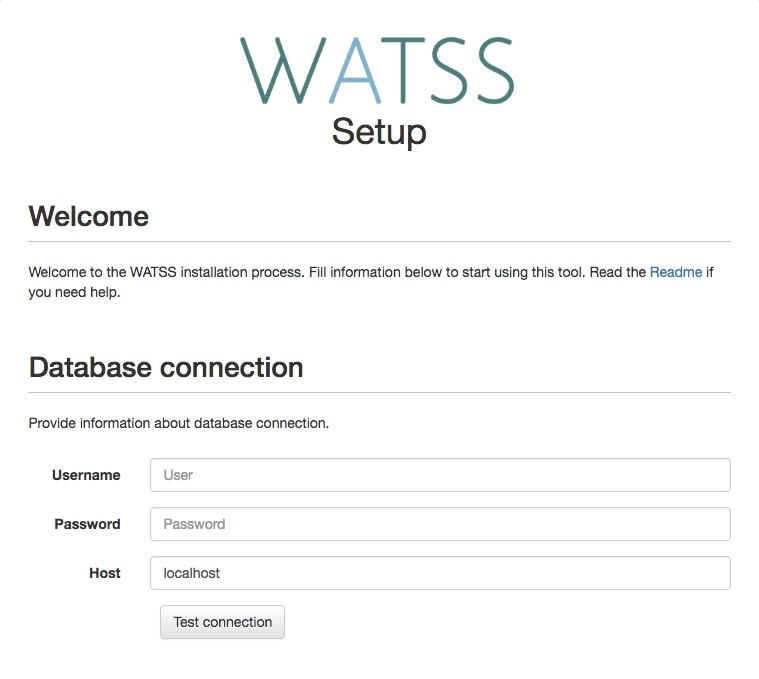
\includegraphics[width=0.8\linewidth]{images/setup1.jpg}
  \caption{Inizio procedura di installazione}
  \label{fig:setup1}
\end{figure}

\subsection{Connessione al database}

Come prima cosa sarà necessario impostare i parametri per la \emph{connessione al database} che verrà utilizzato dall'applicazione. 

Inserite \emph{username}, \emph{password} e \emph{host} del database desiderato. L'utente selezionato deve poter creare nuovi database.

\subsection{Locazione dei frames}

Per procedere è necessario creare una cartella che conterrà i frames nella root dell'applicazione.  All'interno di quest'ultima, creare una cartella per ciascuna camera di cui si posseggono i frames, usando unicamente notazione numerica (per esempio 1, 2, etc.).

In ciascuna cartella così creata inserire i frame relativi alla camera considerata. I frame devono essere ordinati in ordine crescente mediante il nome dell'immagine.

Terminate queste operazioni preliminari inserire il nome della cartella creata inizialmente e selezionare \emph{Verify folder}. Se tutto è andato a buon fine verranno mostrate le camere trovate (come in Figura \ref{fig:setup2}).

\begin{figure}[h]
\centering
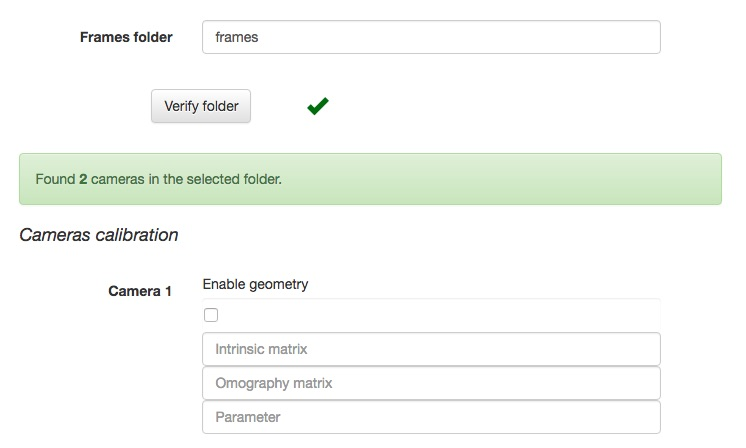
\includegraphics[width=0.8\linewidth]{images/setup2.jpg}
  \caption{Inizializzazione delle camere}
  \label{fig:setup2}
\end{figure}

Per ciascuna camera trovata sarà possibile impostare i parametri per la calibrazione.

\subsection{Ultime configurazioni}

Il passo successivo dell'installazione consiste nella selezione del database. E' necessario inserire il nome del database che si vuole utilizzare, se questo non è presente verrà automaticamente creato.

Come ultimo passaggio, inserire la lista di utenti con cui sarà possibile accedere all'applicazione. E' necessario specificare almeno un utente.

Terminate queste operazioni, premere su \emph{Install WATSS}. Se la procedura guidata va a buon fine verrà notificato tramite una pagina di conferma.

